\documentclass[10pt,a4,oneside]{article}
\usepackage{a4wide}
\usepackage{graphicx}


\newenvironment{mylisting}
{\begin{list}{}{\setlength{\leftmargin}{1em}}\item\scriptsize\bfseries}
{\end{list}}

\newenvironment{mytinylisting}
{\begin{list}{}{\setlength{\leftmargin}{1em}}\item\tiny\bfseries}
{\end{list}}


\begin{document}

\title{COMPSCI 7096B - Software Engineering Group Project}
\author{Milestone 4 - Group 1}
\date{Mon Aug 18, 2008}

\maketitle

\section*{Ticket 186 - Daemon Remove Feature}

\paragraph{} By Filimoni Lutunaika (1154924)

\paragraph{}


\subsection*{Introduction}

The Earth daemon operates by monitoring the size and file constituency of 
selected directories. This functionality requires the daemon to be able to 
add and remove monitored directories on-the-fly. The daemon can add 
directories to be monitored but the feature to remove or cease monitoring 
directories had yet to be implemented. The only way to remove directories 
was to access and directly manipulate the backend database.


\paragraph{}

\subsection*{Task Description}

Ticket 186 proposes the actual implementation of the remove directory 
feature and the relevant provisions already exists in the Earth daemon 
code. In fact, the daemon script recognises the remove option as a valid 
command but simply indicated that the feature is not functional. This 
existing deficiency provides the basis for investigating how this feature 
can be effectively integrated into the existing codebase.



\newpage

\subsection*{Implementation}

\paragraph{}
To help ensure that the implementation of the remove feature is consistent 
with the original vision of the Earth project developers, the investigative 
tasks focussed initially on identifying the existing implementation of the 
add feature. 


\paragraph{}
First, the following modifications were made to the Earth daemon code:


\begin{figure}[h!]
\begin{centering}
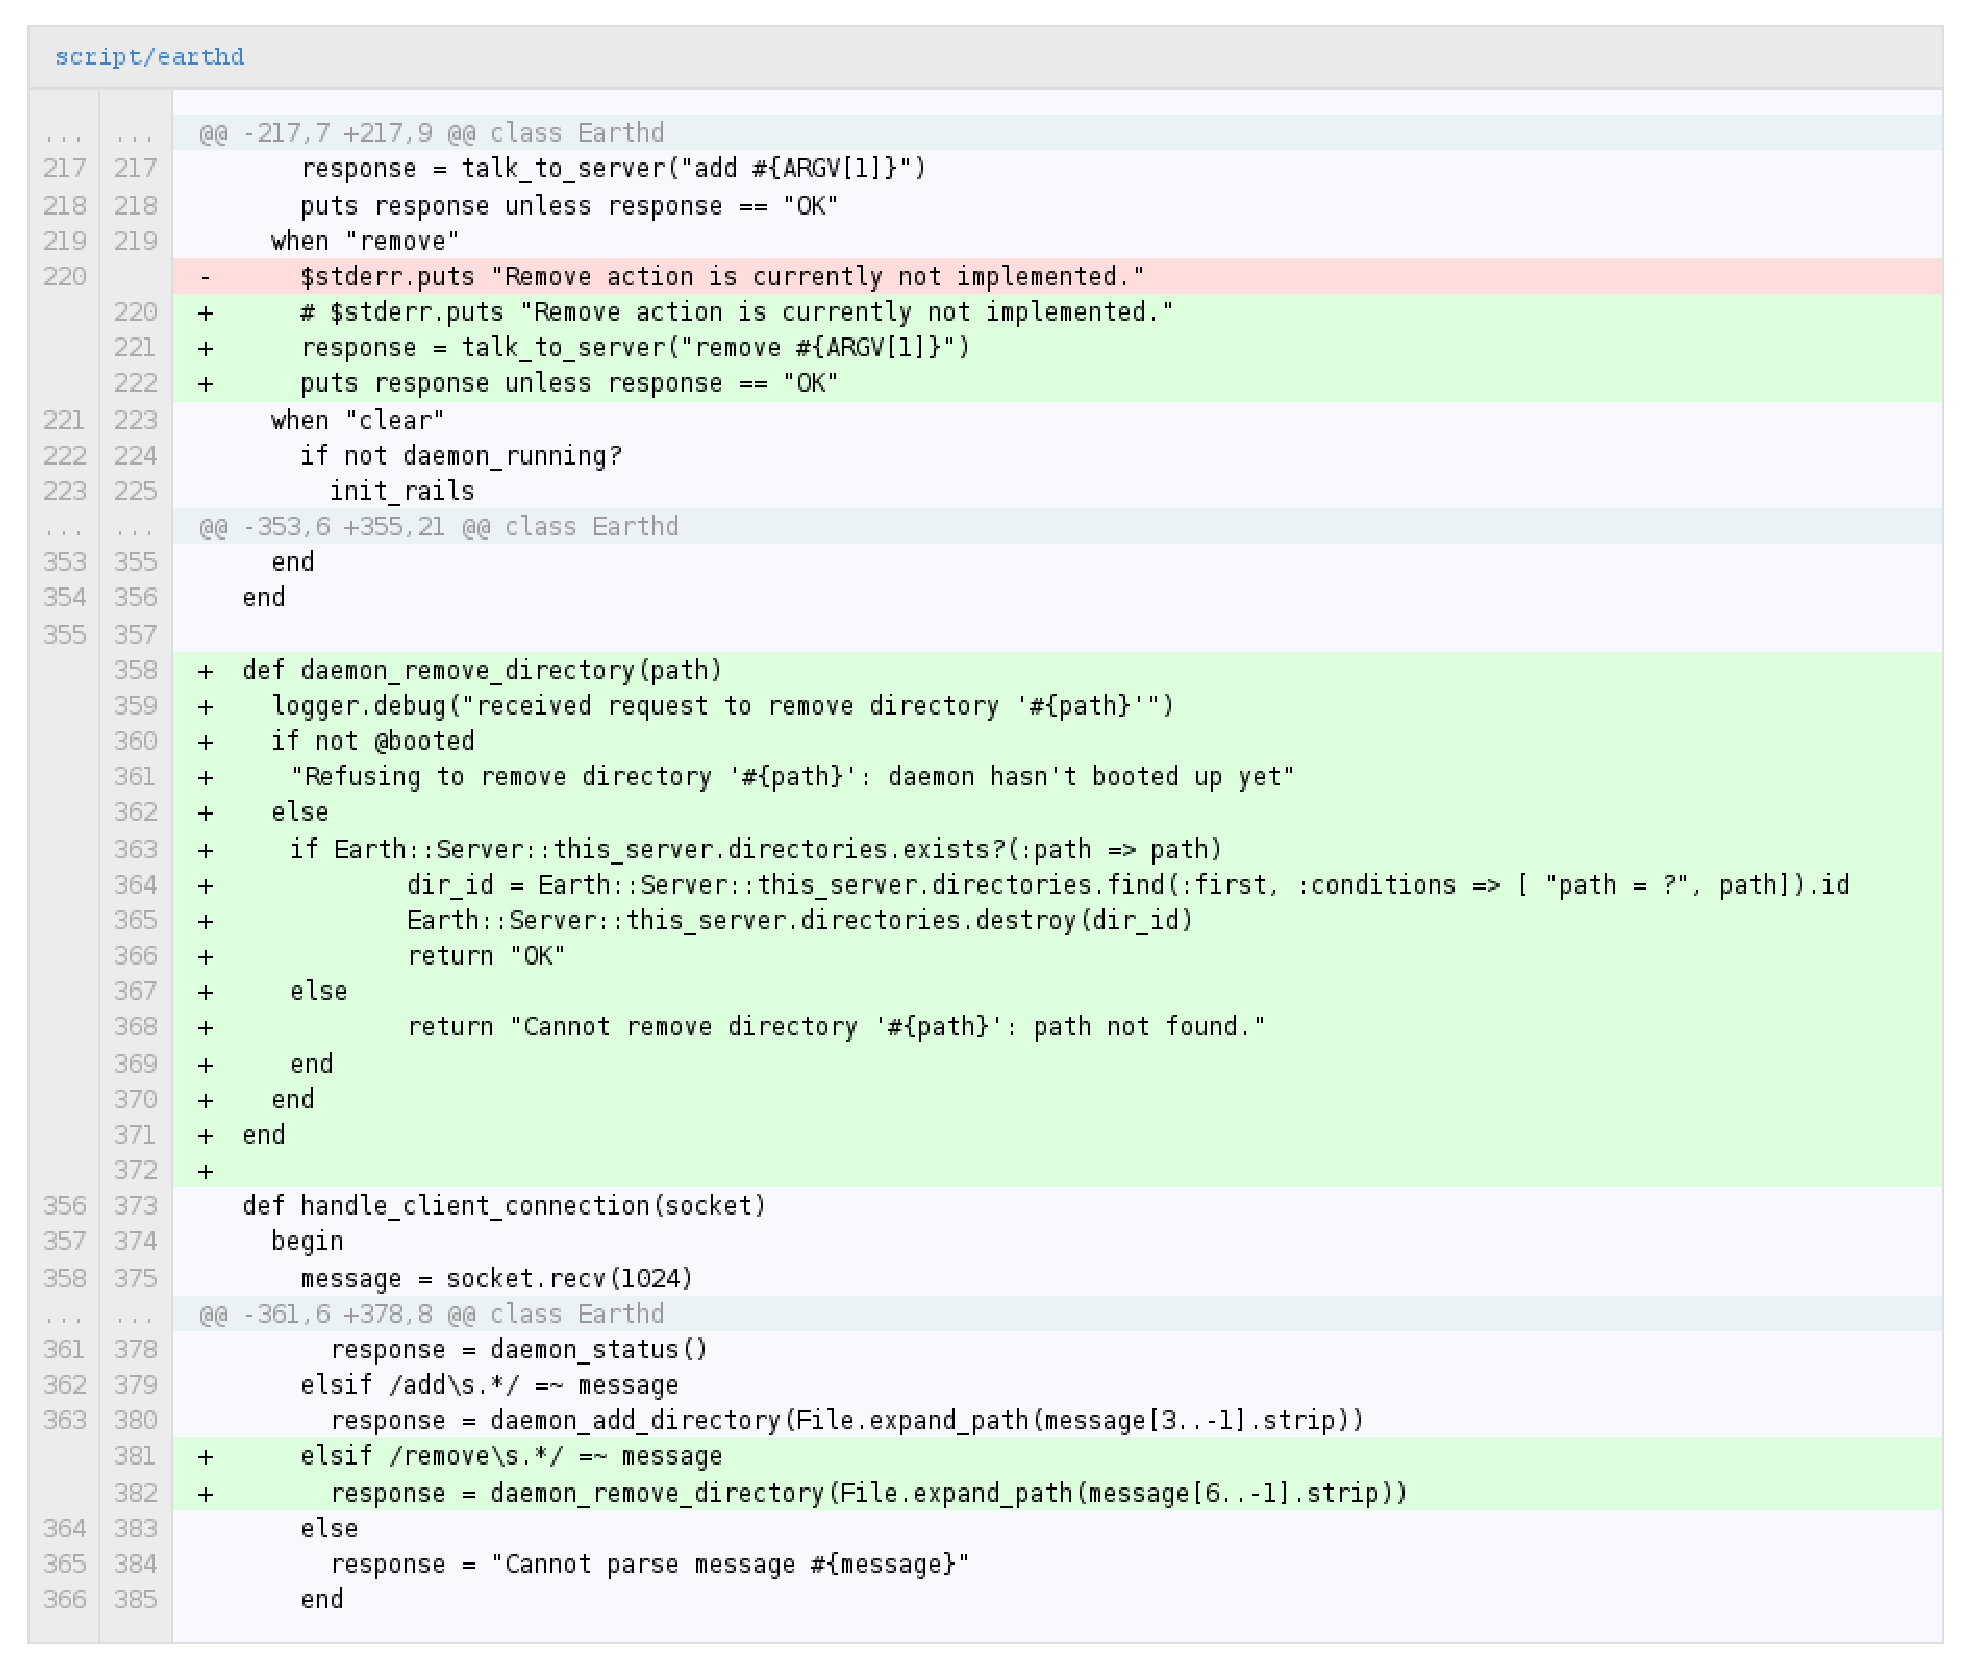
\includegraphics[width=150mm]{figs/earthd}
\end{centering}
\caption{Daemon code modification.}
\label{fig:earthd}
\end{figure}


\paragraph{Note:}
The added code snippets are highlighted green while the removed code 
snippets are highlighted red.


\newpage

\paragraph{}
Further modifications were then made to the code to ensure that the given 
path name is a valid directory as shown below.

\begin{figure}[h!]
\begin{centering}
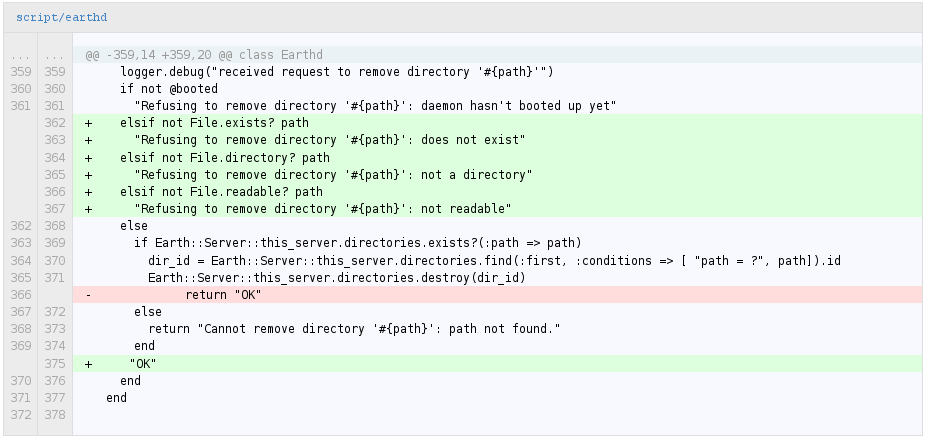
\includegraphics[width=150mm]{figs/earthd2}
\end{centering}
\caption{Validating directory path.}
\label{fig:earthd2}
\end{figure}


\newpage

\paragraph{}
The following changes were then made to the model, controller and view 
codes respectively to enable the execution of the directory removal 
feature from the web-based user interface.


\begin{figure}[h!]
\begin{centering}
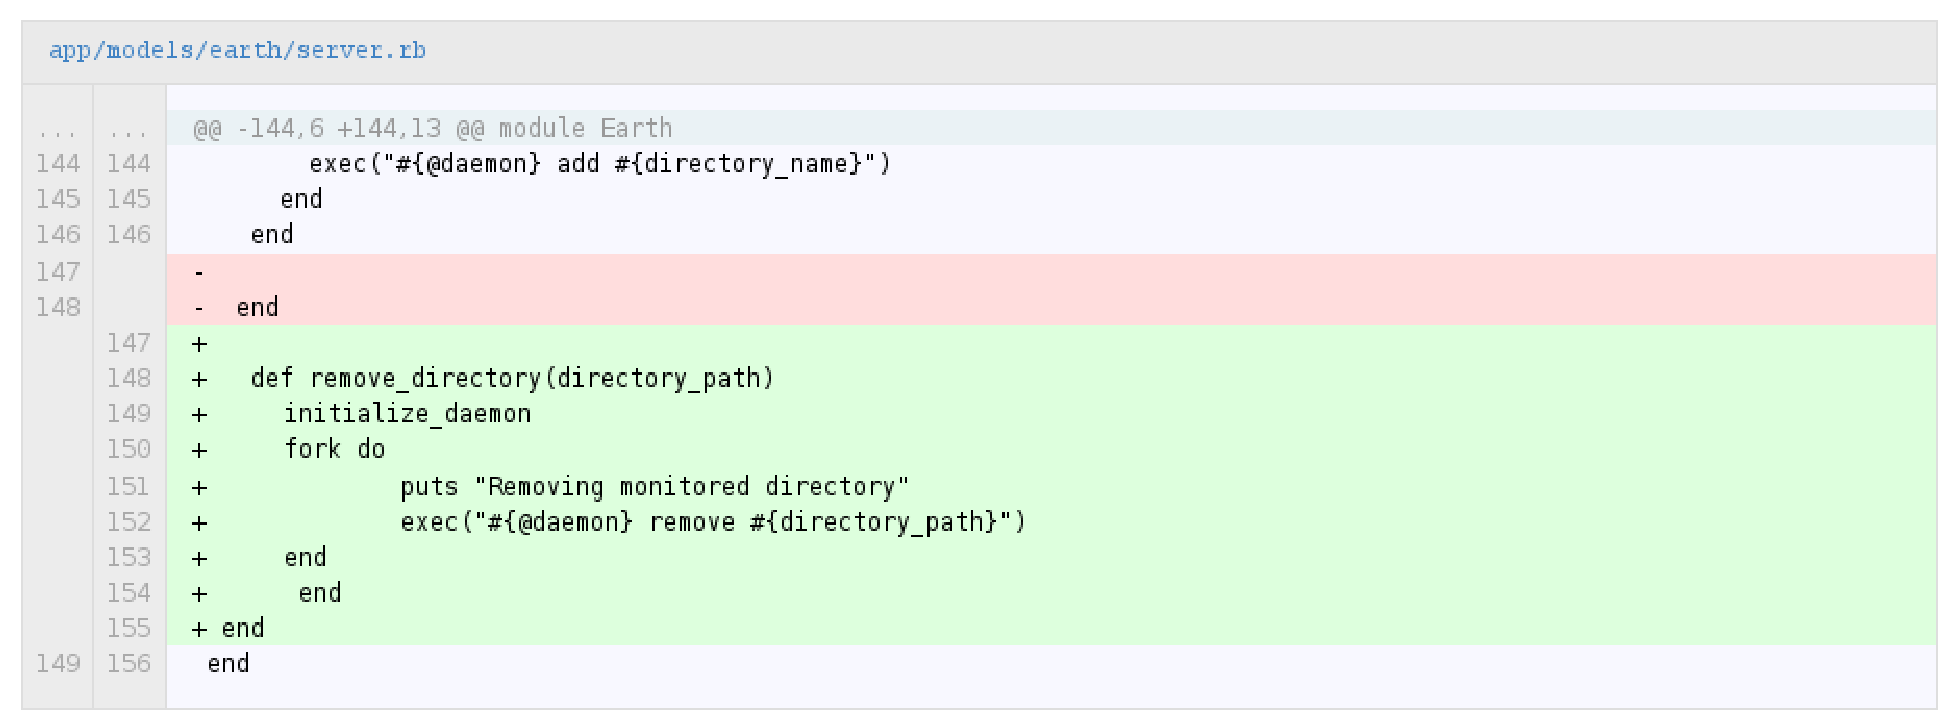
\includegraphics[width=150mm]{figs/earthmodel}
\end{centering}
\caption{Modified model code.}
\label{fig:earthmodel}
\end{figure}


\begin{figure}[h!]
\begin{centering}
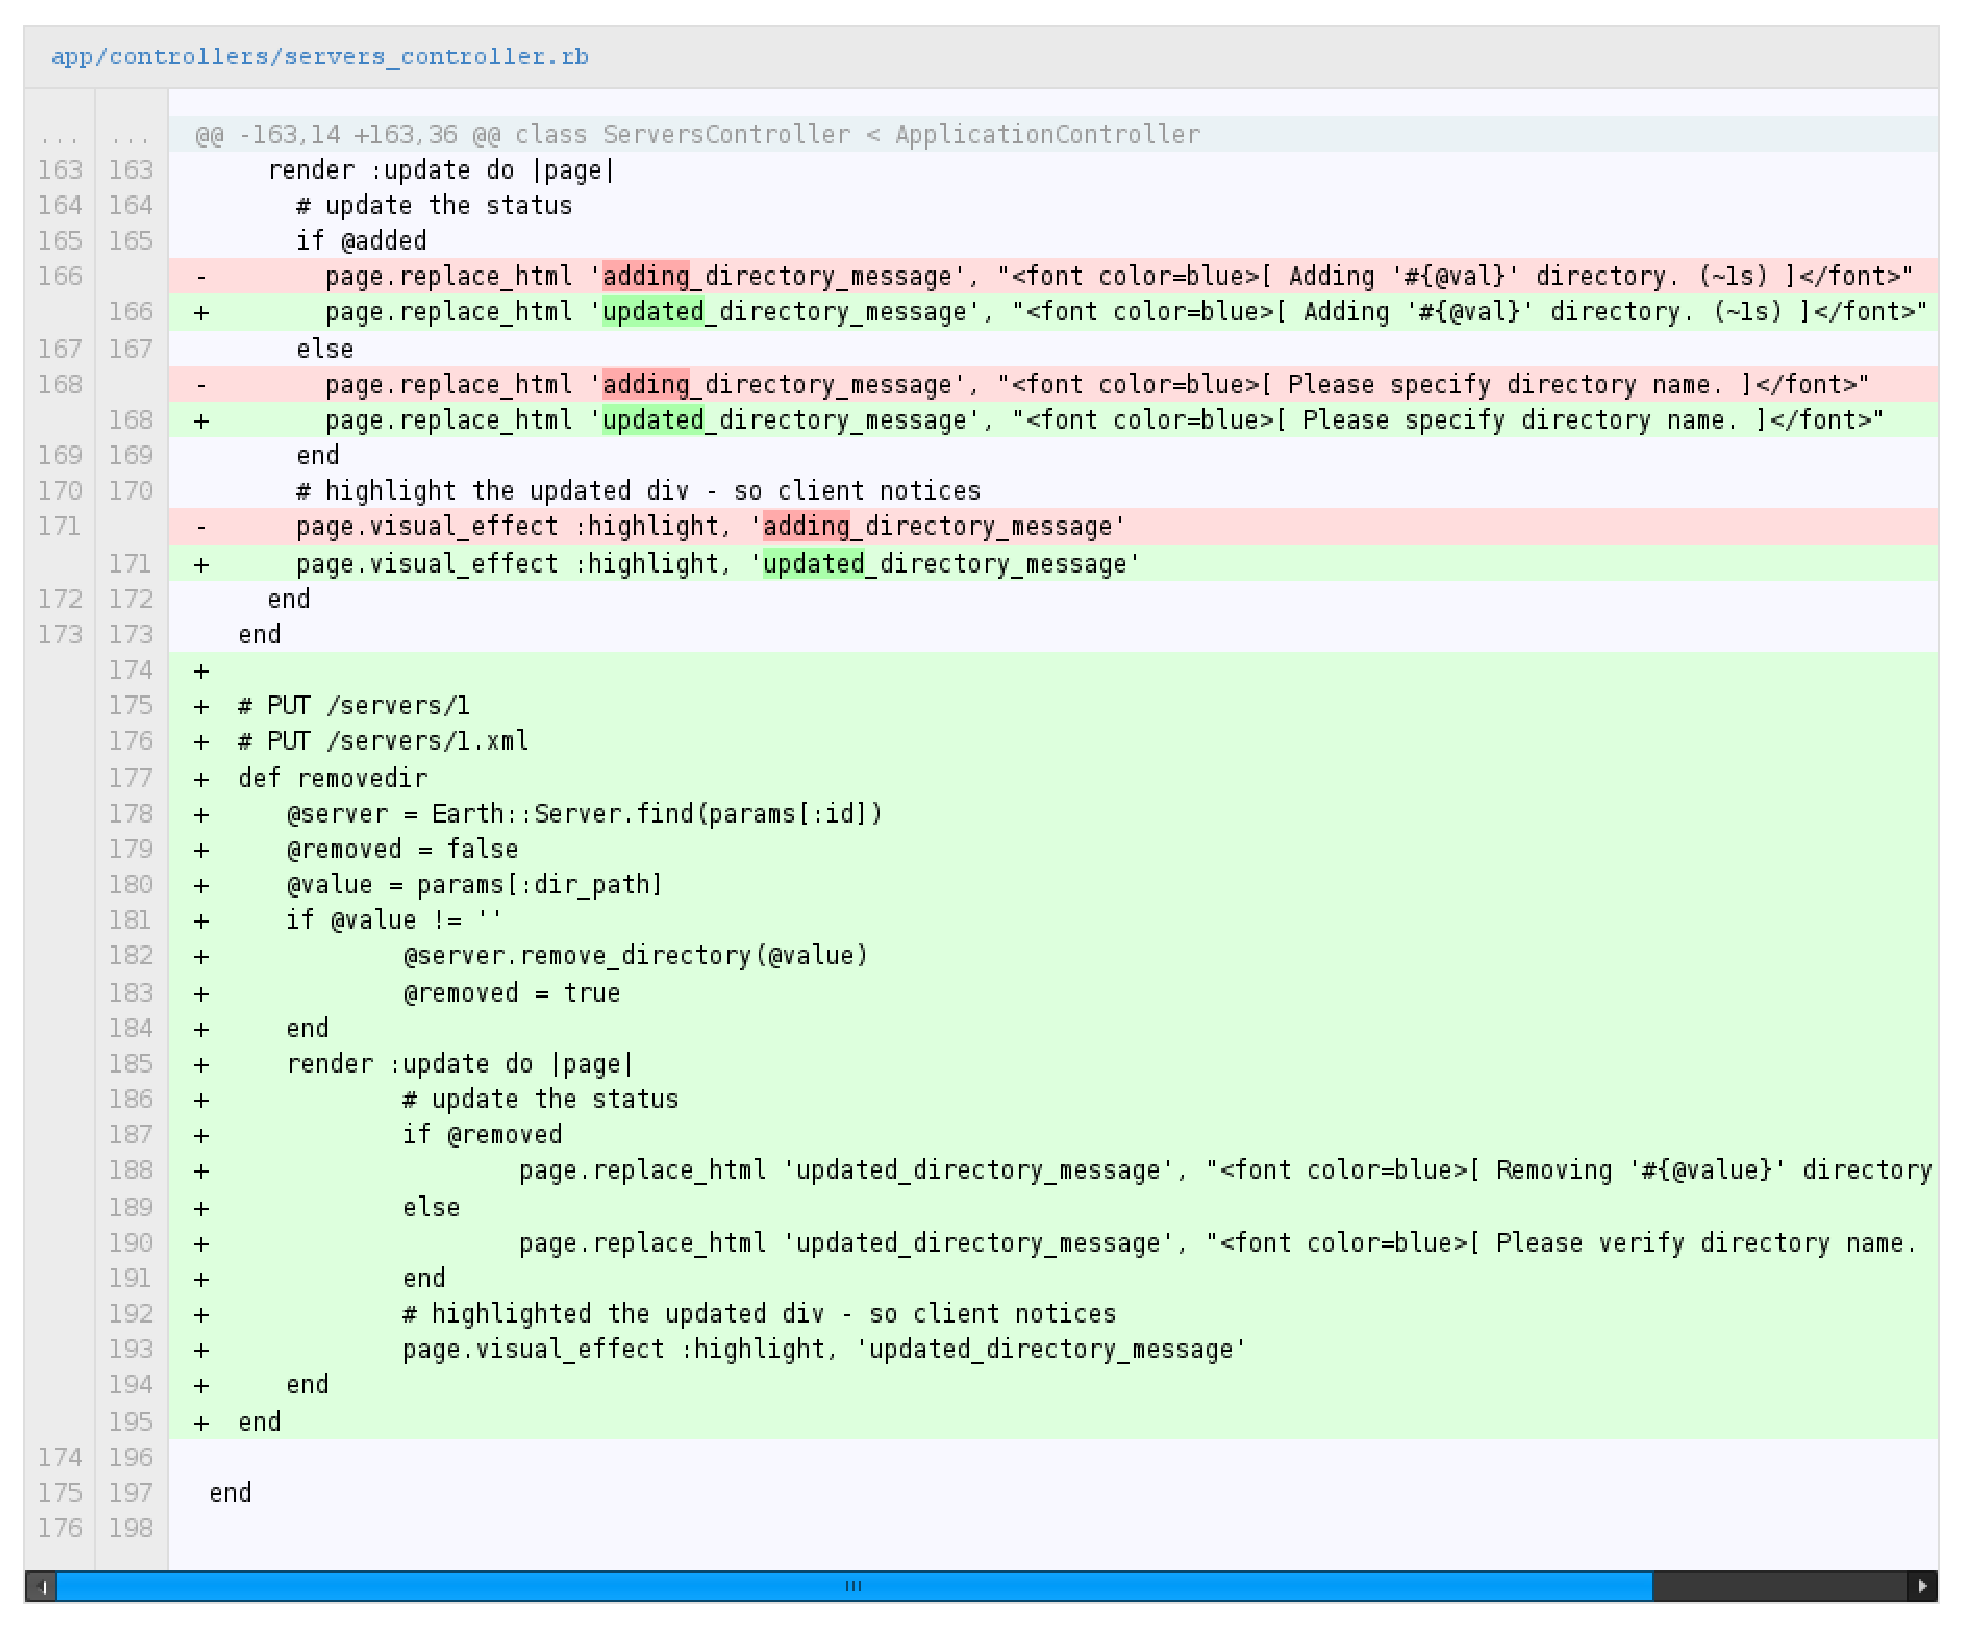
\includegraphics[width=150mm]{figs/earthcontroller}
\end{centering}
\caption{Modified controller code.}
\label{fig:earthcontroller}
\end{figure}


\begin{figure}[h!]
\begin{centering}
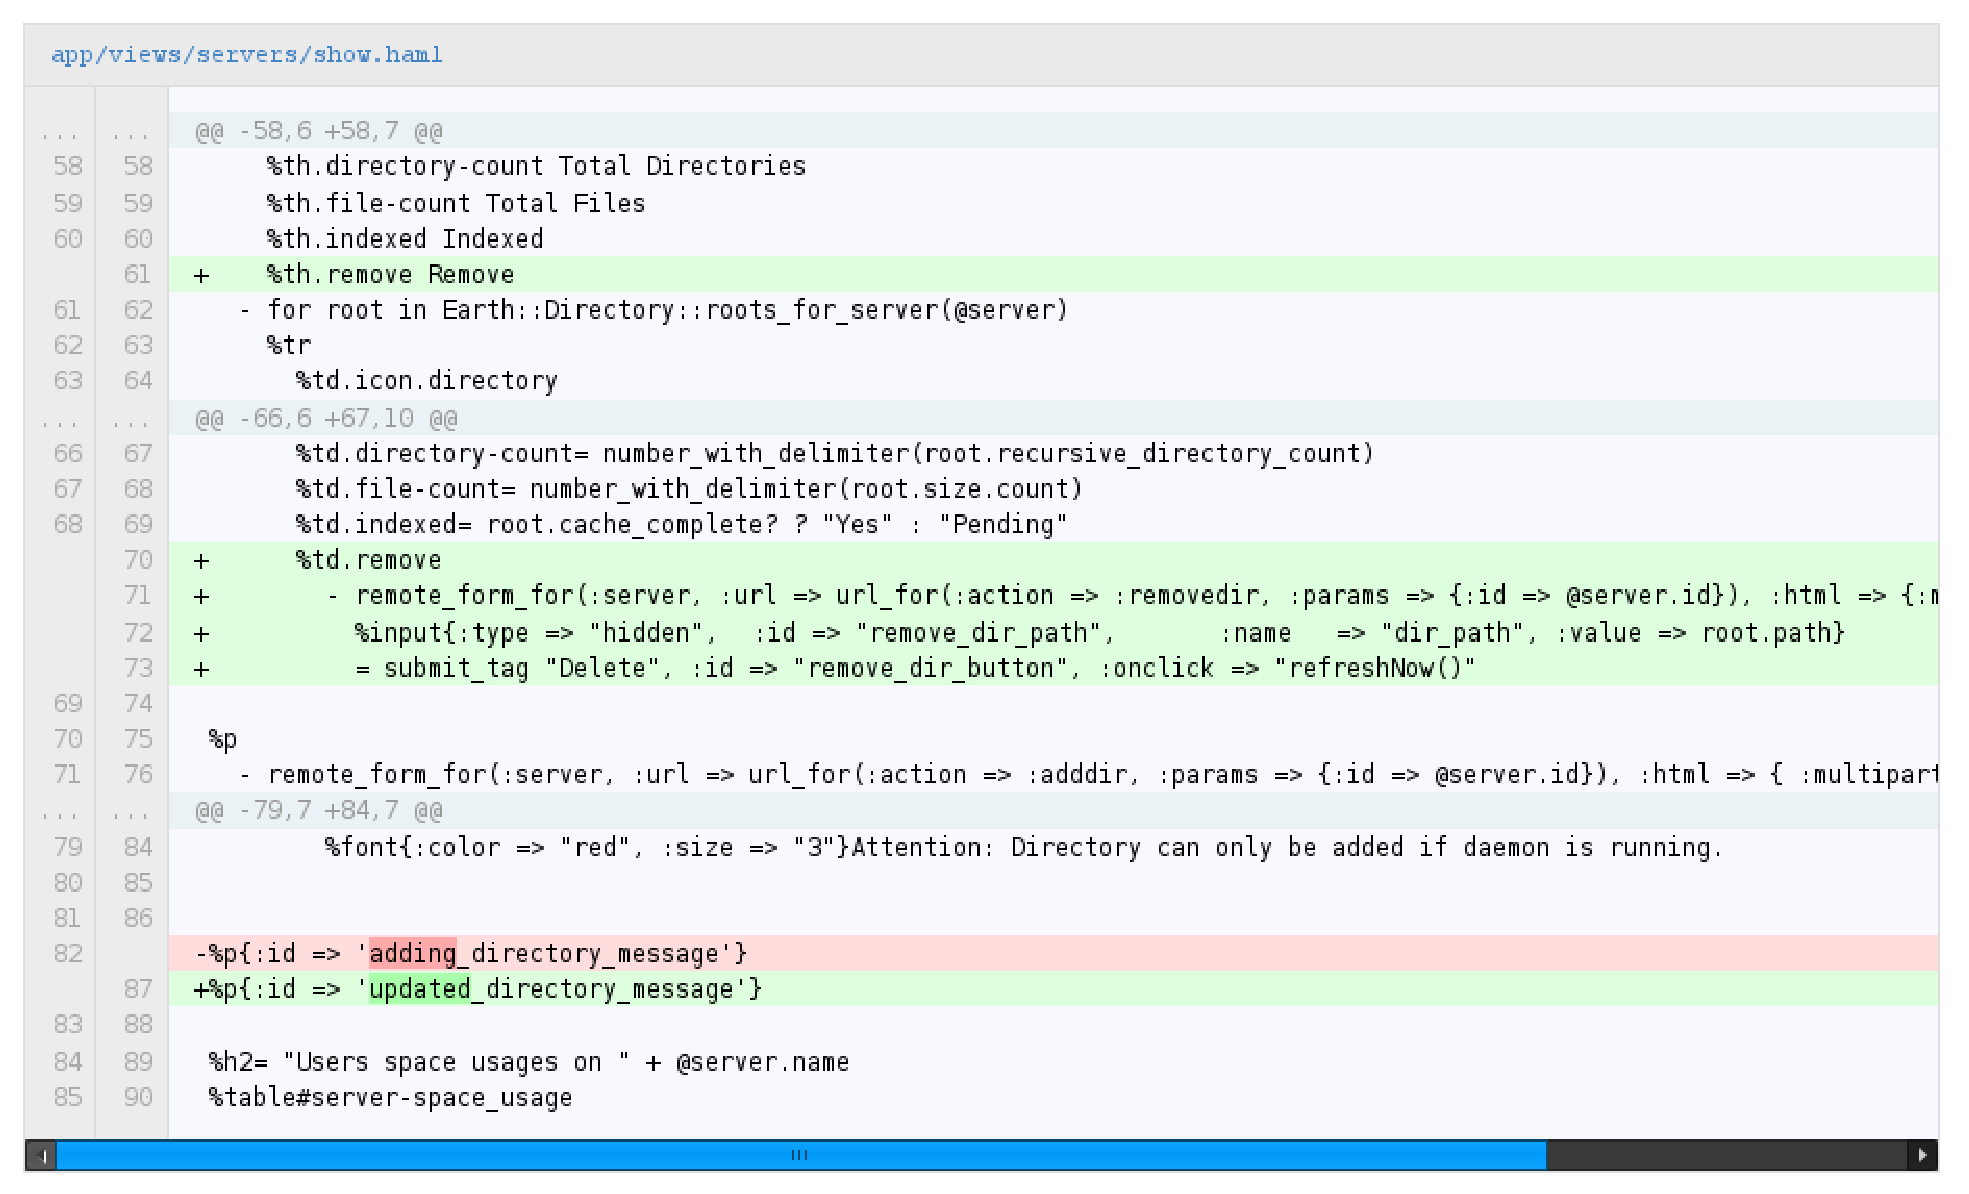
\includegraphics[width=150mm]{figs/earthview}
\end{centering}
\caption{Modified view code.}
\label{fig:earthview}
\end{figure}



\newpage

\paragraph{}
The following additional modification was then made to the view code 
to sort the list of monitored folder in ascending alphabetical order.


\begin{figure}[h!]
\begin{centering}
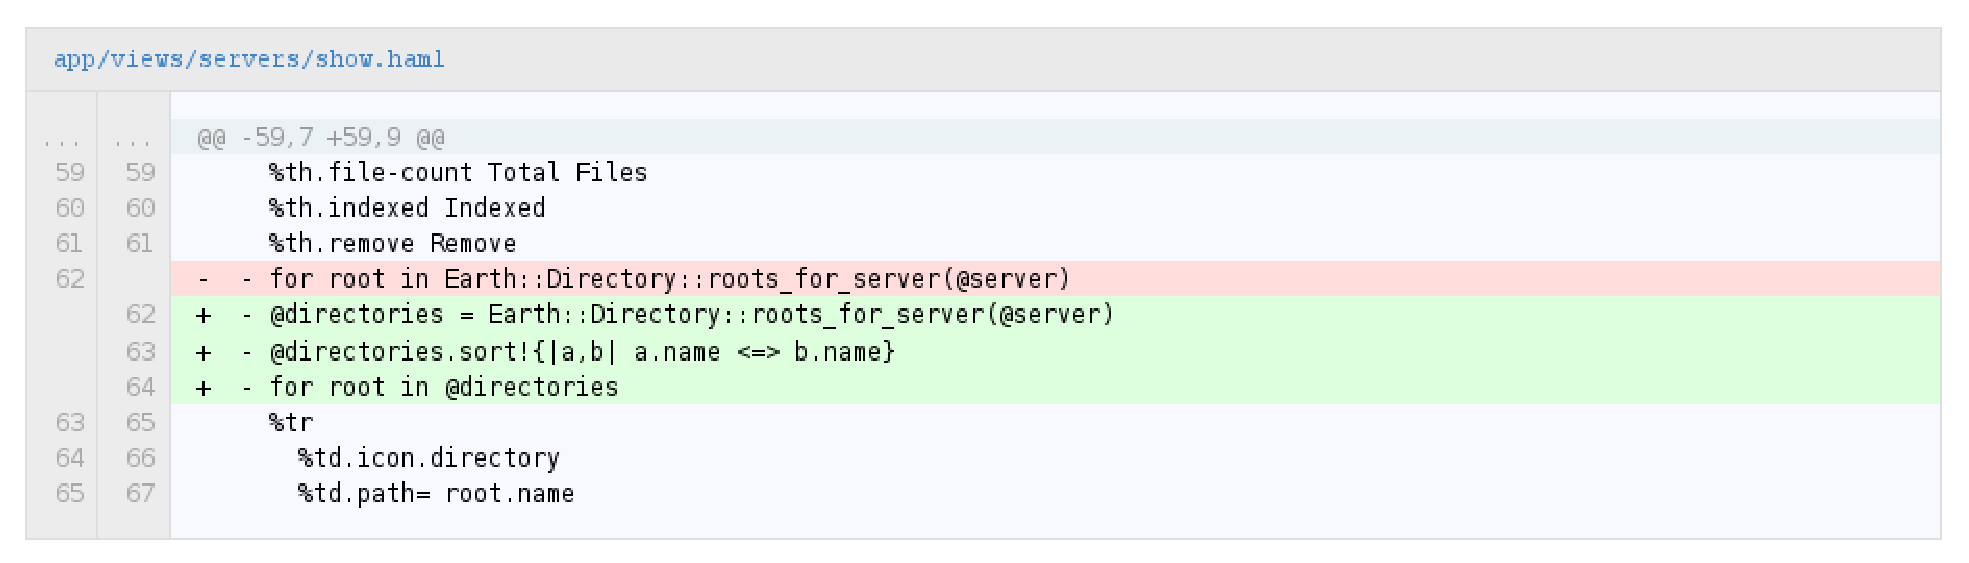
\includegraphics[width=150mm]{figs/earthshow2}
\end{centering}
\caption{Modified view code to sort directory listing.}
\label{fig:earthshow2}
\end{figure}


\newpage

\paragraph{}
Unfortunately, these changes would cause the unexpected termination 
of the daemon whenever the remove method is invoked. Apparently, the 
removal action introduced some inconsistencies between the cached 
data and the directories array which would trap the daemon on 
subsequent updates. The following modification was then made to the 
file monitor plugin to resolve this data consistency issue.



\begin{figure}[h!]
\begin{centering}
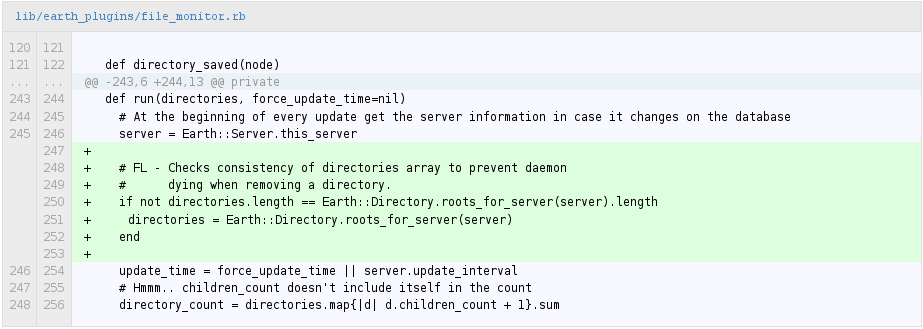
\includegraphics[width=150mm]{figs/filemonitor}
\end{centering}
\caption{Modified file monitor code to resolve data inconsistency.}
\label{fig:filemonitor}
\end{figure}


\paragraph{}
These changes effectively enabled the resulting implementation of 
the daemon remove feature. Further, these code modifications were 
pushed onto the remote github repository (ssurfer/earth.git) before 
it would be further propagated onto the Group 1 repository 
(segp2sg1/earth.git).



\newpage

\subsection*{Results}

\paragraph{}
Apart from the code snippets presented in the previous section, 
the only other visual outcome of this task were the delete buttons 
column on the monitored directories listing as shown in the 
following screenshot.


\begin{figure}[h!]
\begin{center}
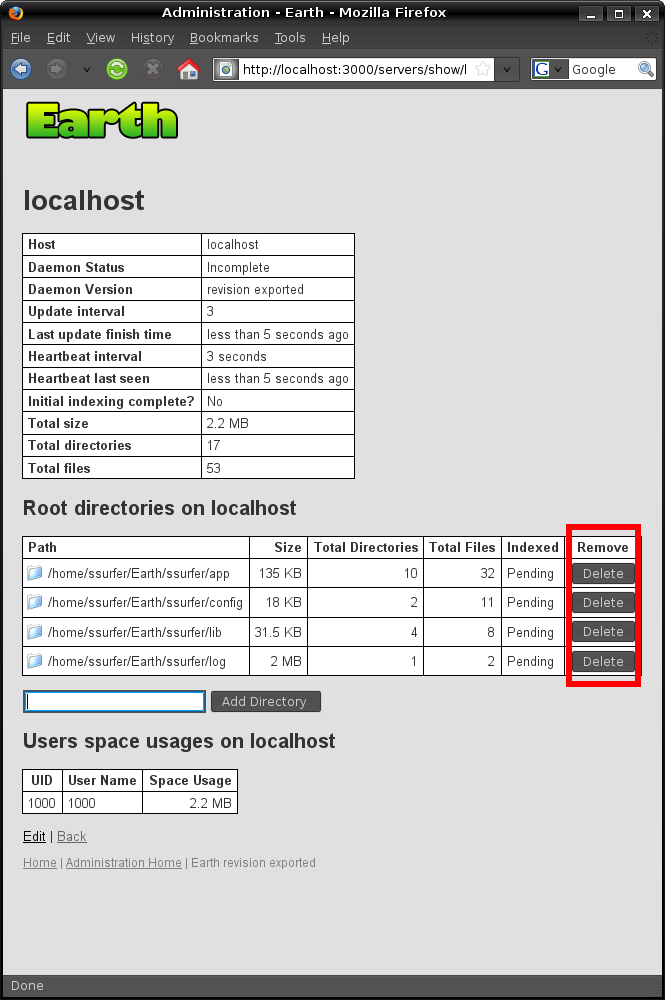
\includegraphics[width=90mm]{figs/screendel}
\end{center}
\caption{Directory listing with delete column.}
\label{fig:screendel}
\end{figure}


\newpage

\subsection*{Discussion}

\paragraph{}
For this task, the allocated time of 81 hours was adopted based 
on the feedback from Milestone 3 wherein a preliminary study was 
conducted. This time was subdivided into the following subtasks in 
the Milestone 4 Plan document:

\begin{enumerate}
\item Investigate the existing add feature of the daemon. (8hrs)
\item Identify the relevant components of the remove feature. (16hrs)
\item Design and code an effective implementation of the remove feature. (40hrs)
\item Test and integrate solution to the Subgroup 1 codebase. (16hrs)
\item Update the Earth Trac system. (1hr)
\end{enumerate}

\paragraph{}
The actual recorded work took 87 hours (log included as Appendix) which in 
hindsight, appeared to have been over budgeted for a relatively minor and 
isolated task. However, the task assumed an intermediate level of Ruby On Rails 
understanding and in-depth knowledge of the earth application. 
This particular skillset was limited at the commencement of this current 
milestone and a significant amount of resources (time) had to be expanded 
in order to complete the planned task. Nevertheless, a significant 
understanding of the earth application was attained as a result which 
would certainly be valuable for proceeding with the more challenging 
tasks of later milestones.

\paragraph{}

\subsection*{Conclusion}

\paragraph{}
The daemon remove feature was implemented with appropriate modifications 
in relevant files on the Earth project codebase. Further, a simple 
adaptation of the remove feature on the web user interface was included 
for completeness.

\paragraph{}

\subsection*{Acknowledgement}


\paragraph{}
The code snippets included in this document were extracted using the 
source view feature of the github repositories where the project 
codebase is controlled and distributed.

\paragraph{}


\newpage

\subsection*{Appendix - Development Log}

\paragraph{Note}
Figures rounded to nearest hour in some cases and every effort made 
to keep this log as accurate and informative as possible.

\begin{mylisting}
\begin{verbatim}

Semester 2 Week 1


Monday Jul 28, 2008

1300 - 1500 hrs

Attended main group meeting and discussed planned tasks for Milestone 4.

Daily Total: 2 hrs


Tuesday Jul 29, 2008

0800 - 1100 hrs

Drafted Milestone 4 plan for Group 1 and discussed resource planning with other group members.

1500 - 1700 hrs

Completed and submitted Milestone 4 plan for Group 1.

Daily Total: 5hrs


Wednesday Jul 30, 2008

0800 - 1100 hrs

Investigate implementation of add directory feature.

1300 - 1600 hrs

Revisit rails documentation on ActiveRecord::Base class. (Ref: The Rails Way)

1900 - 2100 hrs

Trace add directory implementation code through the application.

Daily Total: 8 hrs


Thursday Jul 31, 2008

0800 - 1100 hrs

Advanced Rails Tutorial (Ref: Wrox Beginning Rails).

1230 - 1530 hrs

Continued with Advanced Rails Tutorial (Ref: Wrox Beginning Rails).

Daily Total: 6 hrs


Friday Aug 1, 2008

0800 - 1100 hrs

Continued with Advanced Rails Tutorial (Ref: Wrox Beginning Rails).

1300 - 1600 hrs

Revisited earth code on add directory feature and identified remove feature components on MVC framework.

Daily Total: 6 hrs


Weekly Total:  27 hrs
========================================================================




Semester 2 Week 2


Monday Aug 4, 2008

1300 - 1400 hrs

Attended main group meeting and discussed progress.

1600 - 1900 hrs

Continued with coding as planned design had to revised.

Daily Total: 4 hrs


Tuesday Aug 5, 2008

1300 - 1600 hrs

Code and progressively test the remove feature implementation.

1800 - 2100 hrs

Continued with coding.

Daily Total: 6 hrs


Wednesday Aug 6, 2008

1400 - 1500 hrs

Attended Group 1 subgroup meeting with Dr. Li.

1800 - 2100 hrs

Continued with the coding. Delete method still doesn't work.

Daily Total: 4 hrs


Thursday Aug 7, 2008

0800 - 1100 hrs

Continued with coding.Monday Aug 3, 2008

1900 - 2200 hrs

Continued with coding.

Daily Total: 6 hrs


Friday Aug 8, 2008

1300 - 1600 hrs

Revisited base class to find out the SQL statement of the delete and delete_all method.

1800 - 2200 hrs

Still no luck with actual removal action.

Daily Total: 6 hrs


Weekly Total:  26 hrs
========================================================================









Semester 2 Week 3

Sunday Aug 10, 2008

1000 - 1400 hrs

Tested various methods in ActiveRecord::Base class to identify most suitable removal method.

1600 - 1800 hrs

Identified the 'destroy' class method in ActiveRecord::Base as the best option to remove directory 
for the daemon.

Daily Total: 6 hrs


Monday Aug 11, 2008

1300 - 1400 hrs

Group Meeting at SE Meeting Room

2000 - 0000hrs

Investigated the termination of the daemon when removing a directory. Still not resolved.

Daily Total: 5 hrs


Tuesday Aug 12, 2008

1200 - 1530 hrs

Traced through daemon execution sequence to identify termination condition.

1700 - 2330 hrs

Continued with above unresolved task.

Daily Total: 10 hrs


Wednesday Aug 13, 2008

1000 - 1500 hrs

Devised test script to trap daemon execution sequence. Found 'culprit' code in file monitor 
plugin module (file_monitor.rb).

Daily Total: 5 hrs


Thursday Aug 14, 2008

2000 - 2300 hrs

Verified conformance of remove feature with existing unit tests.

Daily Total: 3 hrs


Friday Aug 15, 2008

0800 - 1000 hrs

Repeated unit and function tests. Updated remote group 1 repository (segp2sg1/earth.git).

1130 - 1330 hrs

Tested repository code on uni machine and prepared for group presentation.

1400 - 1500 hrs

Attended milestone 4 presentation.

Daily Total: 5 hrs


Weekly Total: 34 hrs
========================================================================


\end{verbatim}
\end{mylisting}

\[----\]
\end{document}
